\documentclass[french,]{article}
\usepackage{lmodern}
\usepackage{amssymb,amsmath}
\usepackage{ifxetex,ifluatex}
\usepackage{fixltx2e} % provides \textsubscript
\ifnum 0\ifxetex 1\fi\ifluatex 1\fi=0 % if pdftex
  \usepackage[T1]{fontenc}
  \usepackage[utf8]{inputenc}
\else % if luatex or xelatex
  \ifxetex
    \usepackage{mathspec}
  \else
    \usepackage{fontspec}
  \fi
  \defaultfontfeatures{Ligatures=TeX,Scale=MatchLowercase}
\fi
% use upquote if available, for straight quotes in verbatim environments
\IfFileExists{upquote.sty}{\usepackage{upquote}}{}
% use microtype if available
\IfFileExists{microtype.sty}{%
\usepackage{microtype}
\UseMicrotypeSet[protrusion]{basicmath} % disable protrusion for tt fonts
}{}
\usepackage[margin=1in]{geometry}
\usepackage{hyperref}
\hypersetup{unicode=true,
            pdfborder={0 0 0},
            breaklinks=true}
\urlstyle{same}  % don't use monospace font for urls
\ifnum 0\ifxetex 1\fi\ifluatex 1\fi=0 % if pdftex
  \usepackage[shorthands=off,main=french]{babel}
\else
  \usepackage{polyglossia}
  \setmainlanguage[]{french}
\fi
\usepackage{graphicx,grffile}
\makeatletter
\def\maxwidth{\ifdim\Gin@nat@width>\linewidth\linewidth\else\Gin@nat@width\fi}
\def\maxheight{\ifdim\Gin@nat@height>\textheight\textheight\else\Gin@nat@height\fi}
\makeatother
% Scale images if necessary, so that they will not overflow the page
% margins by default, and it is still possible to overwrite the defaults
% using explicit options in \includegraphics[width, height, ...]{}
\setkeys{Gin}{width=\maxwidth,height=\maxheight,keepaspectratio}
\IfFileExists{parskip.sty}{%
\usepackage{parskip}
}{% else
\setlength{\parindent}{0pt}
\setlength{\parskip}{6pt plus 2pt minus 1pt}
}
\setlength{\emergencystretch}{3em}  % prevent overfull lines
\providecommand{\tightlist}{%
  \setlength{\itemsep}{0pt}\setlength{\parskip}{0pt}}
\setcounter{secnumdepth}{0}
% Redefines (sub)paragraphs to behave more like sections
\ifx\paragraph\undefined\else
\let\oldparagraph\paragraph
\renewcommand{\paragraph}[1]{\oldparagraph{#1}\mbox{}}
\fi
\ifx\subparagraph\undefined\else
\let\oldsubparagraph\subparagraph
\renewcommand{\subparagraph}[1]{\oldsubparagraph{#1}\mbox{}}
\fi

%%% Use protect on footnotes to avoid problems with footnotes in titles
\let\rmarkdownfootnote\footnote%
\def\footnote{\protect\rmarkdownfootnote}

%%% Change title format to be more compact
\usepackage{titling}

% Create subtitle command for use in maketitle
\newcommand{\subtitle}[1]{
  \posttitle{
    \begin{center}\large#1\end{center}
    }
}

\setlength{\droptitle}{-2em}
  \title{}
  \pretitle{\vspace{\droptitle}}
  \posttitle{}
  \author{}
  \preauthor{}\postauthor{}
  \date{}
  \predate{}\postdate{}


\begin{document}

\begin{centering}

\vspace{6 cm}

\Huge

{\bf LSINF2275 : Projet 1 : Processus de décision markovien }

\vspace{1 cm}

\large


\vspace{2 cm}

\Large
Mise en application d'un processus de décision markovien avec le jeu de l'oie
\vspace{5 cm}


\Large
Guillaume Truffaut et Patrick Guerin


\vspace{5 cm}

\Large
1 avril 2018

\vspace{3 cm}



\normalsize
Université Catholique de Louvain

\vspace{3 cm}



\end{centering}

\graphicspath{ {(C:/Users/Guillaume/Documents/GitHub/markov-processes/} }

\newpage

`\tableofcontents'

\newpage

\usepackage[francais]{babel}

\section{1. Introduction et explication du jeu
(Guillaume)}\label{introduction-et-explication-du-jeu-guillaume}

L'objectif du projet est de mettre en application les processus de
décision markovien sur un jeu de l'oie modifié. Ce dernier est modélisé
de la manière suivante :

\begin{figure}[h]
\caption{Schéma du jeu de l'oie modifié}
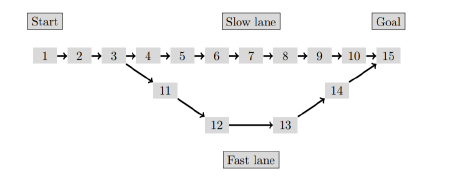
\includegraphics{jeu de l'oie.PNG}
\centering
\end{figure}

\section{2. Théorie : algorithme d'itération de la valeur
(Patrick)}\label{theorie-algorithme-diteration-de-la-valeur-patrick}

\section{3. Simulation du jeu
(Guillaume)}\label{simulation-du-jeu-guillaume}

\section{4. Adaptation du jeu}\label{adaptation-du-jeu}

\section{4.1 Ajout d'une prison
(Patrick)}\label{ajout-dune-prison-patrick}

\section{4.2 Adaptation de la pénalité d'une case (cost sensitive
?)}\label{adaptation-de-la-penalite-dune-case-cost-sensitive}

\section{5. Conclusion}\label{conclusion}


\end{document}
